\begin{sidewaysfigure}
  \centering
  \begin{minipage}{.8\textwidth} % adjust the width as needed

    \begin{minipage}{0.5\textwidth}
      \centering
      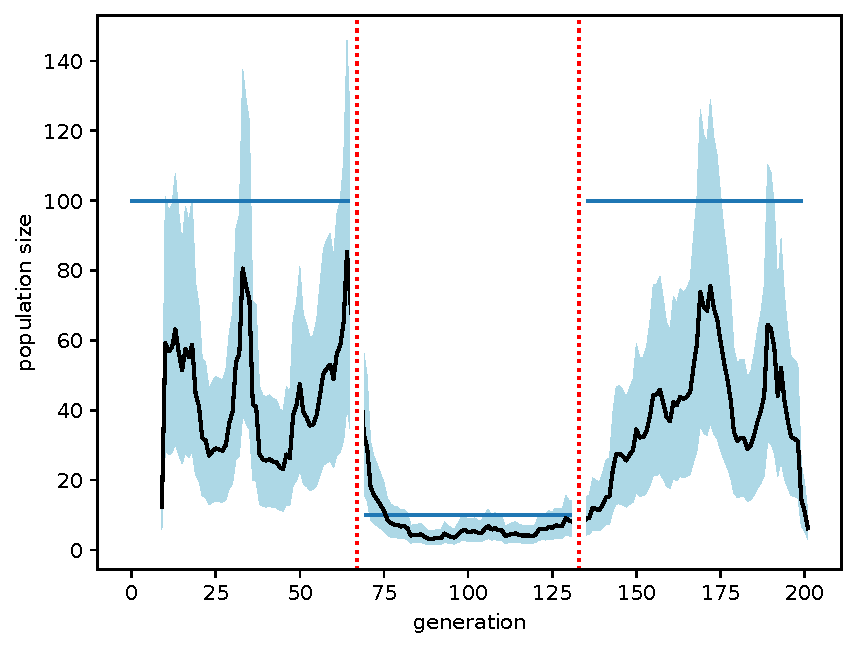
\includegraphics[height=0.3\textheight]{notebooks/notebooks/teeplots/notebook=ne-inference+replicate=0+treatment=bottleneck+viz=plot-running-estimation+x=rank+y=population-size+ext=}
      \subcaption{Bottleneck treatment}
      \label{fig:ne-example-replicates:bottleneck}
    \end{minipage}%
    \begin{minipage}{0.5\textwidth}
      \centering
      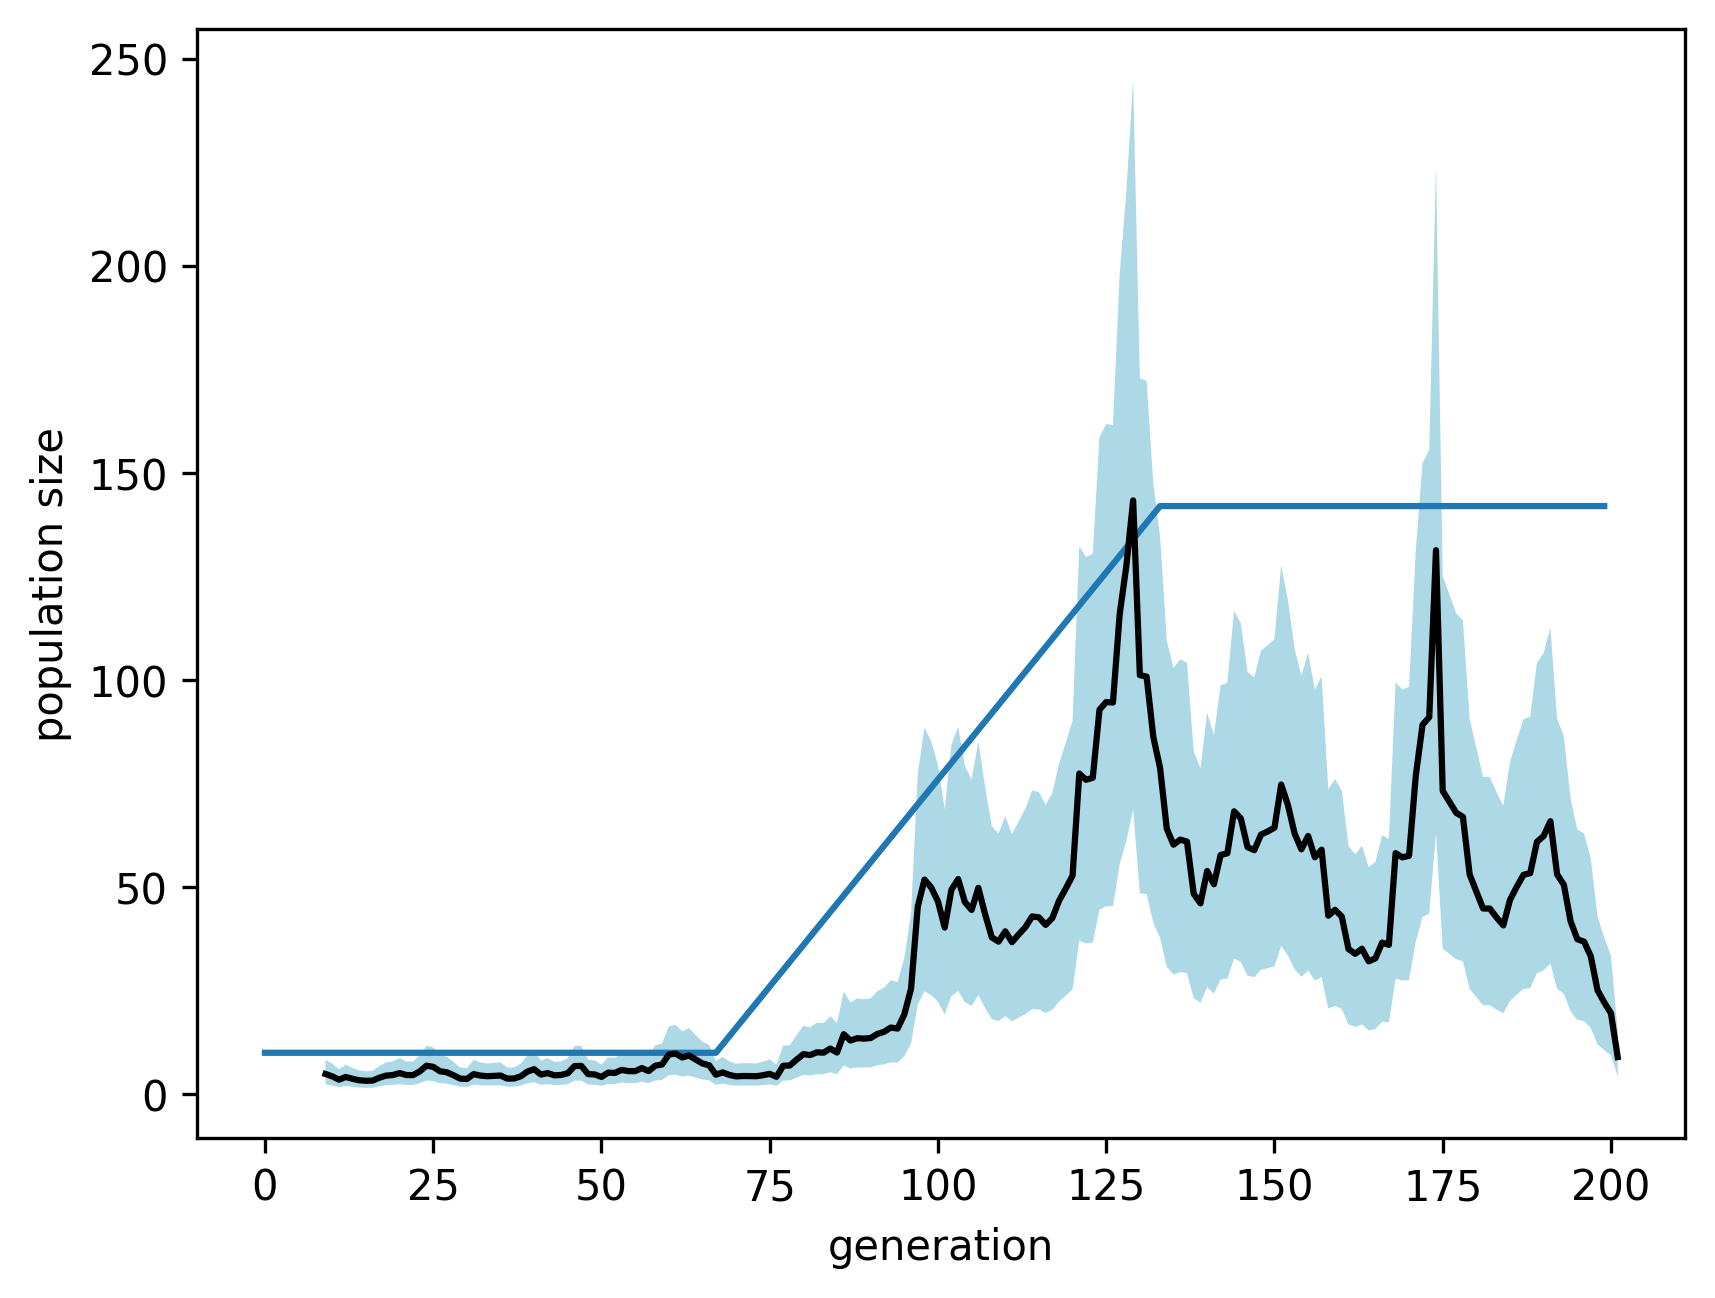
\includegraphics[height=0.3\textheight]{notebooks/notebooks/teeplots/notebook=ne-inference+replicate=0+treatment=range-expansion+viz=plot-running-estimation+x=rank+y=population-size+ext=}
      \subcaption{Range expansion treatment}
      \label{fig:ne-example-replicates:range_expansion}
    \end{minipage}

    \vspace{1cm}

    \begin{minipage}{0.5\textwidth}
      \centering
      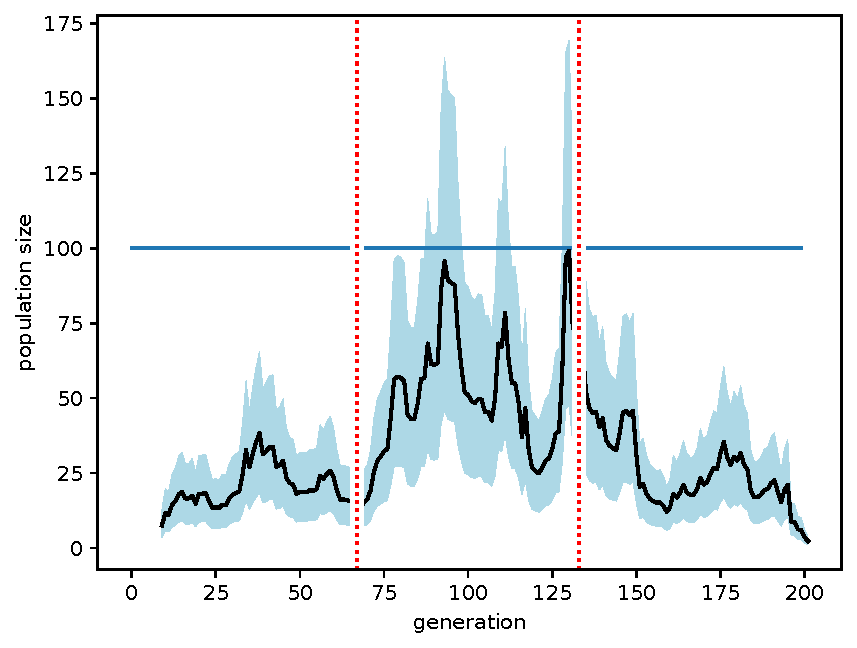
\includegraphics[height=0.3\textheight]{notebooks/notebooks/teeplots/notebook=ne-inference+replicate=0+treatment=selection-pressure+viz=plot-running-estimation+x=rank+y=population-size+ext=}
      \subcaption{Selection pressure treatment}
      \label{fig:ne-example-replicates:selection_pressure}
    \end{minipage}%
    \begin{minipage}{0.5\textwidth}
      \centering
      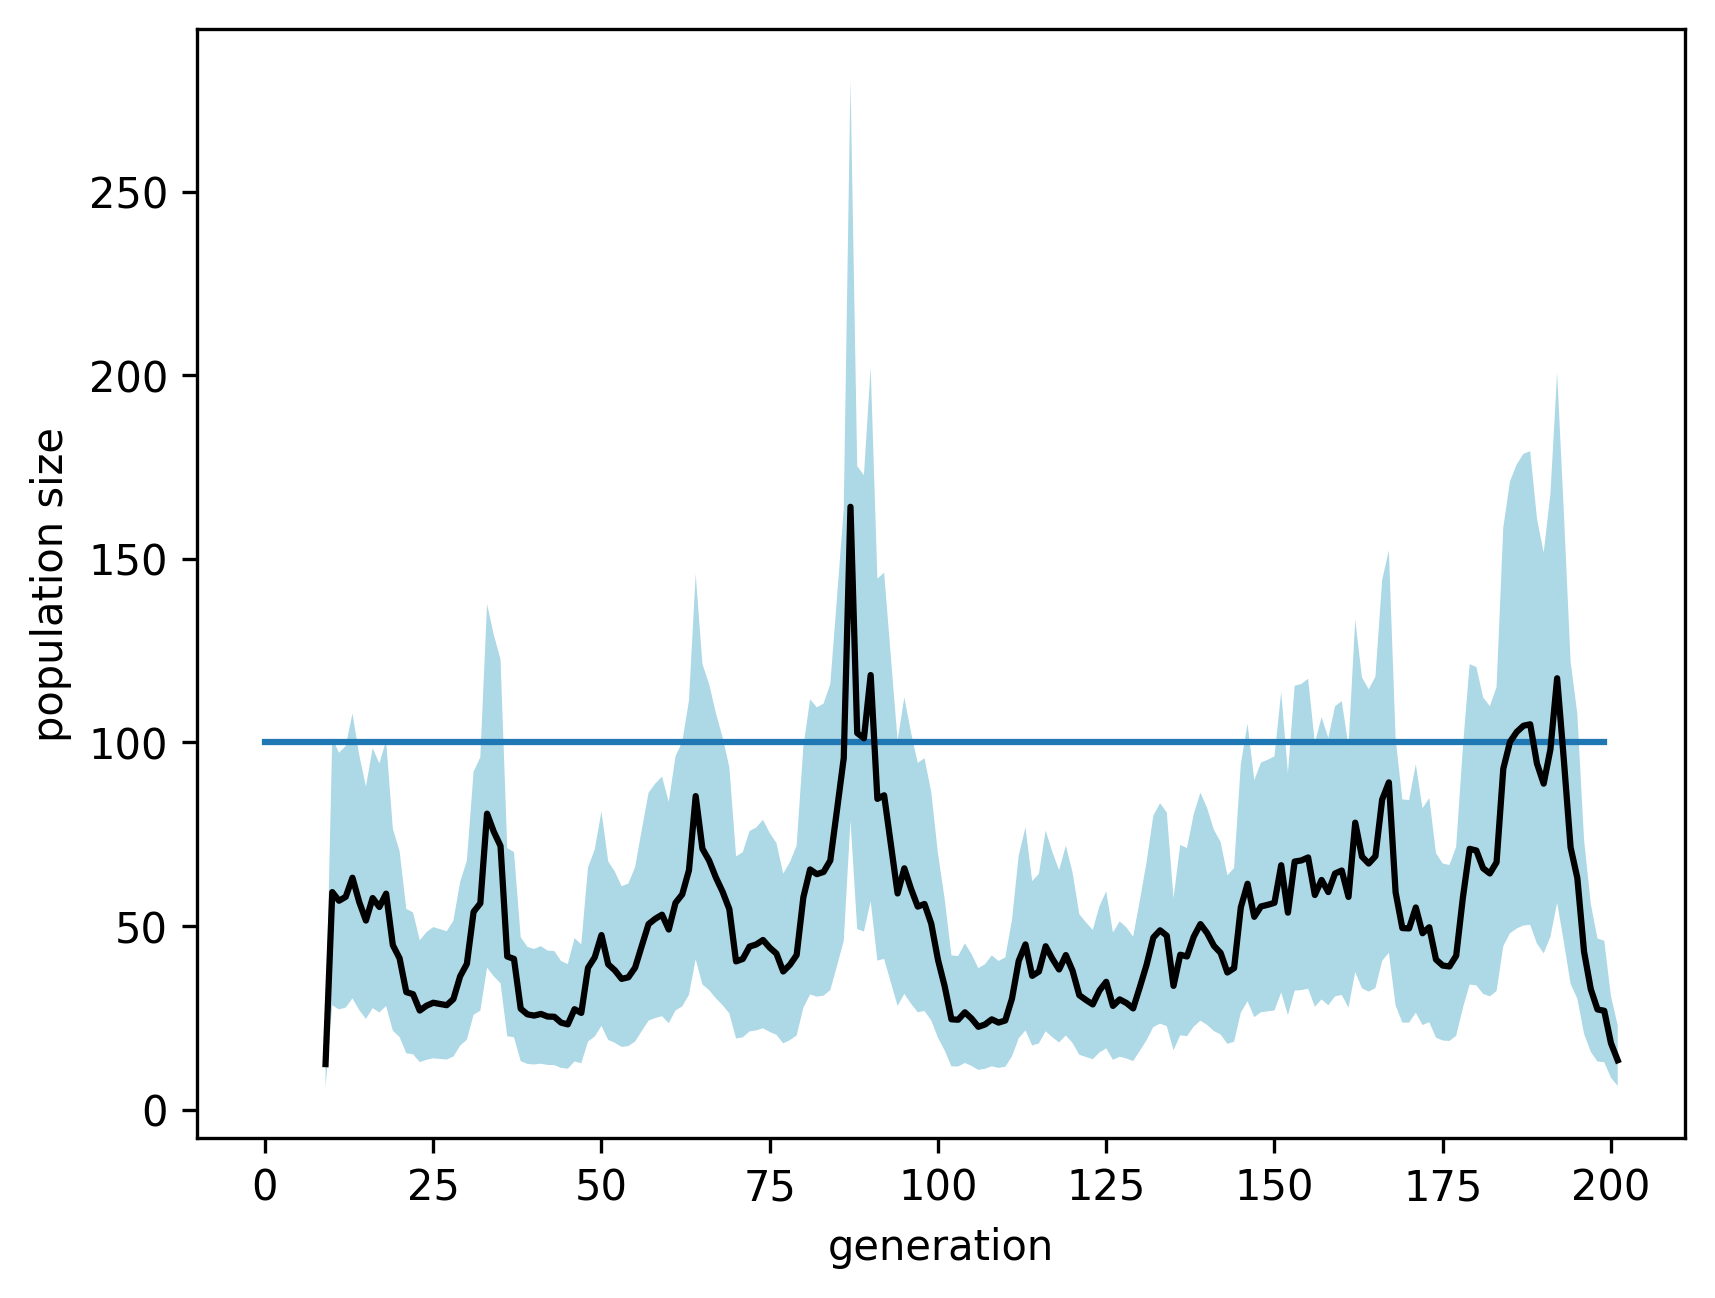
\includegraphics[height=0.3\textheight]{notebooks/notebooks/teeplots/notebook=ne-inference+replicate=0+treatment=control+viz=plot-running-estimation+x=rank+y=population-size+ext=}
      \subcaption{Control treatment}
      \label{fig:ne-example-replicates:control}
    \end{minipage}

  \end{minipage}
  \hfill % Creates horizontal space. Can also use \hspace{<len>}
  \begin{minipage}{.15\textwidth} % adjust the width as needed
    \caption{Ten-sample running MLE estmate of effective population size of example replicates from  each treatment.
    Shaded region corresponds to 95\% MLE confidence interval.
    Horizontal blue lines indicate true population size.
    Dashed vertical lines indicate treatment discontinuities.
    See Section \ref{sec:population-size-inference-experiments} for population size and selection pressure manipulations performed for each treatment.
    Note that disparity between estimated effective population size and true population size is expected due to demographic factors depressing effective population size.
    }
    \label{fig:ne-example-replicates}
  \end{minipage}

\end{sidewaysfigure}


% notebooks/notebooks/teeplots/notebook=ne-inference+replicate=0+treatment=bottleneck+viz=plot-running-estimation+x=rank+y=population-size+ext=.pdf
%
% notebooks/notebooks/teeplots/notebook=ne-inference+replicate=0+treatment=control+viz=plot-running-estimation+x=rank+y=population-size+ext=.pdf
%
% notebooks/notebooks/teeplots/notebook=ne-inference+replicate=0+treatment=range-expansion+viz=plot-running-estimation+x=rank+y=population-size+ext=.pdf
%
% notebooks/notebooks/teeplots/notebook=ne-inference+replicate=0+treatment=selection-pressure+viz=plot-running-estimation+x=rank+y=population-size+ext=.pdf
